\chapter{Програмна реализация}
\section{Избор и изграждане на базата данни}

Една система за езиково обучение очевидно се нуждае, най-малко, от
някакви речникови данни, на които тя да базира своите модули. Тези
данни трябва да бъдат съхраняване някъде. Много подобни системи
съхраняват данните си директно в текствови или двоични файлове. Това,
обаче, не е особено ефективно когато искате да правите произволен
достъп до данните или да манипулирате много от тях едновременно. 

Едно много по-ефективно решение е да се използва вградена релационна
база данни - подход използвам в много популярни приложение, като
Mozilla Firefox(SQLite), OpenOffice.org(HSQLDB) и т.н. В света на Java
приложенията най-популярните вградени бази данни са HSQLDB, H2 и Apache
Derby(изестна още като Java DB). И трите са реализирани изцяло на Java
и се интегрират отлично с Java приложения. В настоящата дипломна работа H2
Database беше предпочетена поради изключително високото си
бързодействие, малкият размер оперативна памет, която тя използва,
отличната си документация, чести обновления и леснота на употреба.

За да бъде тя достъпна в приложението трябва да се изпълнят следните
стъпки: 
\begin{itemize}
  \item h2.jar трябва да бъде добавен в клас пътя на приложението 
  \item за достъп се използва JDBC драйвера org.h2.Driver
  \item използва се URL за достъп до базата от вида
    jdbc:h2:/path/to/file
  \item ако базата не съществува тя ще бъде създадена първия път,
    когато се свържете към нея
\end{itemize} 
\section{Моделиране на базата данни}

Дизайнът на базата данни на приложението е изчистен, интуитивен и
минималистичен. Основните таблици, в които се съхраняват данните му са
само 5 - DICTIONARIES, DICTIONARY\_ENTRIES, STUDY\_SETS,
STUDY\_SET\_ENTRIES, RANK\_ENTRIES и EXAM\_SCORE\_ENTRIES. Всичките
съдържат няколко общи полета - уникален идентификатор(id), дата на
създаване(created), дата на промяна(modified). Общите полета в
таблиците са изразени в Java кода под формата на абстрактен базов
клас, който всичко други класове от бизнес модела разширяват. 

Таблицата DICTIONARIES съдържа следната информация - име на речник,
име на иконката на речника, двата езика, които го
описват(from\_language, to\_language). Добавянето на нов речник в
системата неминуемо минава през добавянето на нов ред в тази таблица. 

Таблицата DICTIONARY\_ENTRIES съдържа в себе си думите на
речниците. Нейните полета включват дума, превод и референция към
речника, който притежава думата. Следва се ествествената логика, че
един речник притежава много думи.

Таблицата STUDY\_SETS съдържа информация за същестуващите набори от
думи за изучаване. Думите от в един набор трябва да бъдат от
единствен речник, затова таблицата притежава референция към речник.

Таблицата STUDY\_SET\_ENTRIES съдържа думи на един набор, които по
същество са просто препратки към DICTIONARY\_ENTRIES. Освен това имаме
и референция към STUDY\_SET таблицата.

В таблицата RANK\_ENTRIES се съдържа рейтинга на думите в даден
език. Думите с висок рейтинг са често срещани, а тези с малък -
рядко. Както бе упомената и в предната глава, таблицата се използва от
изпитния модул за разделяне на думите по трудности, а данните в нея са
базирани на статистически анализ проведен върху различни литературни
творби.

Таблицата EXAM\_SCORE\_ENTRIES служи за съхранение на резултатите от
положените изпити. В нея се съхранява следната информация - използван
речник, име, брой верни отговори, брой грешни отговори и трудност на
изпита. 
\section{Изграждане на потребителският интерфейс}

Приложението има графичен потребителски интерфейс, реализиран
посредством библиотеката Swing на Java. Присъстват типичните за
повечето приложения елементи като лента с менюта (menubar) и лента с
бутони за бърз достъп до фунции(toolbar). Освен това приложението се
интегрира със областта за нотификации на операционната система.

Особено голяма внимание беше отделено на създаването на аткрактивен и
интуитивен дизайн на потребителският интерфейс. Той бе преработвам
изцяло няколко пъти преди да достигне до текущия си вид. За
допълнително удобство на потребителите интерфейсът е достъпен на
български и на английски език(посредством Translator инфраструктурата
на проекта), като е много лесно добавянето на още езици. 

Swing поддържа концепцията на включваеми външни видове(pluggable look
\& feels) - те позволяват на едно Swing приложение да изглежда по
много различни начини - например като Windows приложение, GTK+
приложение и са начин да се стесни пропастта между Swing апликациите и
така наречените native апликации. Spellbook използва включваемите
външни видове и позволява на потребителя да избери този, който му
допада най-много.
\section{Обобщена архитектура на приложението}
\section{Модули на приложението}
Реализацията на приложението е разделена в четири модула - ядро(core),
помощни пособия(utils), Swing компоненти(swing), потребителски
интерфейс(ui). Модулите на приложението са ясно обособени и са
всъщност и Maven модули - относително автономни единици изходен код.  
\subsection{Ядро}
В модула "`Ядро"' е събрана най-общатата и преизползваема логика на
приложението. Тук е реализирана комуникацията с базата данни, бизнес
модела на приложението и логиката, която задвижва инструментите
"`Изпит"', "`Учене на думи"', "`Проверка на правопис"' и т.н. Вътрешно
модула е разделен на Java пакети, в които е групирана свързаната
логика. Модулът "`Потребителски интерфейс"' се нуждае от възможностите
предоставени от модула "`Ядро"'. Следва описание на някои от ключовите
класове в модула "`Ядро"'.

\begin{itemize}
  \item \textbf{Translator}

    Класът Translator предлага възможност за превод на низове на
    различни езици посредством ResourceBundle. Класът се използва
    изключително от потребителският интерфейс, за да реализира
    възможността той да същестува преведен на различни
    езици. Класът транслатор има private конструктор и неговите
    инстанции се създават чрез метод-шабрика(един от шаблоните за
    дизайн). За всеки ResourceBundle съществува точно една инстанция
    от тип Translator. Инстанциите от класа вътрешно се кешират и се
    преизползват, когато са необходими.

    Всички елементи на графичния потребителски интерфейс притежават в
    себе си инстанция от класа, посредством, която те превеждат
    низовете в тях. За промяна на езиковите на стройките е необходимо
    Spellbook да бъде рестартиран - по време на този процес всички
    съществуващи инстанции на класа биват ре-инициализирани с новите
    езикови настройки.
   
  \item \textbf{AbstractEntity}

    Класът AbstractEntity е много важен, тъй като той е базовият клас,
    който разширяват всички класове част от модела на
    приложението. Самият той е доста прост - съдържа само три полета,
    които са общи за всеки бизнес тип, а именно дата на
    създаване(created), дата на промяна(modified), уникален
    идентификационнен номер(id).

\begin{figure}[htbp]
  \caption{Диаграма на класовете от модела на приложението}
  \centering
  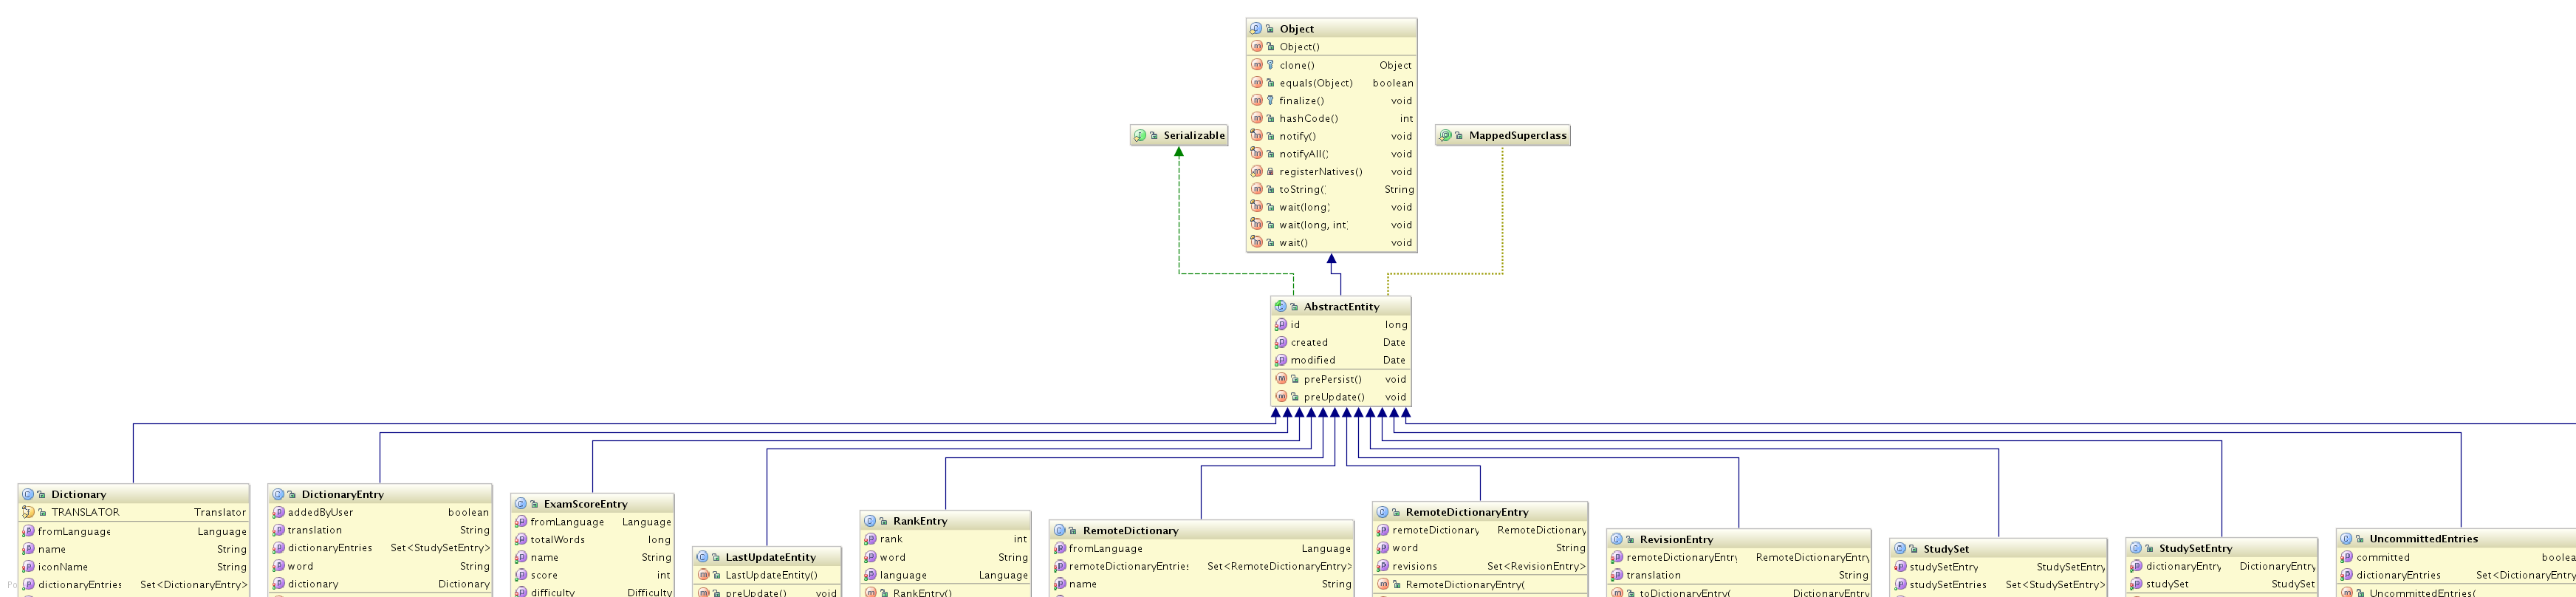
\includegraphics[width=110mm, height=40mm]{images/model-diagram.png}
\end{figure}

  \item \textbf{PreferencesManager}

    Приложението се нуждае от начин за съхранение на потребителските
    настойки между различните сесии и класът PreferencesManager го
    предоставя. Класък представявлява обвивка над стандартния Java
    клас Preferences - всички преференции се записват в единствен
    възел и броят им е ограничен от изброен тип(enum) Preference,
    което елиминира вероятността името на настройка да бъде сбъркана.

    Класът PreferencesManager имплементира шаблона на дизайн
    сек(singleton) - от него съществува единствена инстанция, която си
    споделят всички класове, които имат нужда от него. 

    Самото съхранение на преференциите зависи от операционната
    система, върху която използвате приложението - в Unix базирани
    операционни системи настойките се запазват в скрита папка в
    домашната директория на приложението, а под Windows - в Windows
    регистрите. 

  \item \textbf{AbstractPersistenceService}

    Класът предоставя базов достъп до базата данни на
    приложението. Достъпът се осъществевя посредством единствена
    инстанция от тим EntityManager, която се създава първият път,
    когато се използва класа. Тази инстанция е protected поне на класа
    и това позволява на класовете наследници лесен достъп до
    него. EntityMagager е клас от JPA и той дава възможно за
    извърване на операции създаване, обновяване, изтриване, прочитане
    на персистентни обекти(entities) и за изпълняване на JPQL и SQL
    заявки. Когато имплементацията на JPA, която се използва е
    Hibernate, както в настоящето приложение - класът вътрешно е
    реализиран, използвайки Hibernate Session класа.

    Всички класове, които имат нужда от достъп до базата данни трябва
    да разширяват AbstractPersistenceService. Примери за такива
    класове са DictionaryService, StudyService, ExamService.
  \item \textbf{DictionaryService}

    Класът предоставя достъп до речниците, налични в базата данни и е
    ключов, тъй като други класове, като StudyService и ExamService са
    изградени върху неговите възможните.

    Класът предоставя възможност за извършване на следните операции -
    извеждане на наличните речници, търсене на определен речник,
    изваждане на думите от определен речник, добавене на дума в
    речник, промяна на дума в речник, изтриване на дума от речник,
    проверка за комплементарност на речник, намиране на превод на дума
    от речник, намиране на приблизителен превод на дума от речник.

    Класът комуникира активно с базата данни и затова е естествено, че
    той наследява класът AbstractPersistenceService. Както и другите
    сервизни класове на приложение, DictionaryService е реализиран
    посредством шаблона сек. 

    Интересни подробности в реализацията на класа са воденето на
    подробен журнал(log) за случващите се събития и кеширането на
    речниците в паметта след първоначалото им зареждане. Подробният
    журнал прави лесно проследяването на работата на класа и опроставя
    много процесът на търсене на грешки, които неминуемо
    възникват. Кеширането на речниците пък подобрява многократно
    скороста на превключваме между речниците, които вече са били
    заредени. Първият път речниците трябва да бъдат прочетени от
    базата, която се намира на твърдият диск - това е бавен процес,
    затова копие на речника се казва в асоциативен масив(hash map) в
    оперативната памет. За цената на минимално количество повече памет
    скорост на зареждане на речниците при повторна нужда от тях се
    увеличава буквално в десетки пъти.
  \item \textbf{StudyService}

    Класът предоставя достъп до наборите от думи за учене. Той
    предлага възможност за създаване на набор, добавяне и изтриване на
    думи в него, както и изтриване на набор. Всичките тези операции са
    свързани с базата данни и затова класът разширавя базовия клас
    AbstractPersistenceService. Тъй като думите в наборите са думи от
    речници, класът се нуждае и от DictionaryService, който използва
    вътрешно.

    Както всички сервизни класове на приложението, StudyService е
    реализиран посредством шаблона за дизайн сек и притежава богат
    журнал на изпълнението си.
  \item \textbf{ExamService}

    Класът реализира функционалността необходима за провеждане на
    изпит, а именно разделяне на думите в един речник на нива на
    трудност, предоставяне на думи за изпит, проверка на верността на
    значенията им и записване на крайния резултат от проверждането на
    изпита. 

    Трудностите са дефинирани от изброимия тип Difficulty и имат имена
    и стойности, между които думите се считат за част от дадена
    стойност. Стойностите са определени статистически, чрез анализ на
    дълги художествени текстове на даден език. В процеса се създава
    асоциативна таблицата, ключовете на която са думите, а стойностите
    - броя пъти, в които дадена дума бива срещната. Асоциативния масив
    бива записам в базата данни като таблица(RankEntries). Всички
    получени стойности биват осреднени за да се определят подходящи
    нива за различните трудности. Рядко срещаните думи се маркират
    като трудни, а често срещаните като лесни.

    Преводът на всяка дума има обикновено повече от едно значение. При
    провеждането на изпита потребителя въвежда само по едно значение,
    като отговор на даден въпрос, затова преводите трябва да бъдат
    разделени интелигентно на всички потенциални значения, които могат
    да бъдат приети като отговор. Класът постига това чрез употребата
    на регулярни изрази.

    Тъй като класът достъпва активно базата данни, той също е
    наследник на базовия клас AbstractPersistenceService. Думите,
    използвани в изпитите, са част от речници и затова класът вътрешно
    използва активно инстанцията от класа DictionaryService.

    Както всички сервизни класове на приложението, ExamService е
    реализиран посредством шаблона за дизайн сек и притежава подробен
    журнал на изпълнението си.
  \item \textbf{Spellcheck}
    Функционалността за проверка на правописа е доста комплексна и
    понастоящем притежава две реализации в Spellbook. 

    Оригиналната имплементация е в класа MapSpellChecker и реализира
    прост алгоритъм за проверка на правописа, представен в една от
    статиите на популярният автор и разработчик Питър Норвиг(Peter
    Norvig). Тази имплементация се основа на статистически анализ на
    думите в голям текст на даден език за да се определят
    най-подходящите корекции и използва таблицата RankEntries, която
    се използва още и от ExamService. За съжаление алгоритъма се оказа
    много неефективен откъм употреба на системни ресурси - работи
    бавно и консумира много памет. Затова той бе заменен.

    Новата реализация на проверката на правописа се съдържа в класът
    HunSpellChecker. Той вътрешно използва популярната библиотека за
    проверка на правопис hunspell, използвана още в проекти като
    Google Chrome, OpenOffice.org и Mozilla Firefox. Тази реализация
    използва речниците на hunspell за проверката и работи много
    по-бързо и ефективно от оригиналната. Нейн минус е, обаче, че
    изисква употребата на JNI(Java Native Interface), тъй като
    hunspell е С библиотека и това донякъде нарушава портативността на
    приложението - налага се разпространението на различни негови
    версии, компилирани за различните процесорни микроархитектури.
    
    Както всички сервизни класове на приложението, MapSpellCheck и HunSpellCheck са
    реализирани посредством шаблона за дизайн сек и притежават подробен
    журнал на изпълнението си.
  \item \textbf{CodeHostingService}

    Класът предлага интеграция с услугите, предоставяни от Google Code
    и в частност възможност за създаване на доклад за грешка в
    системата за следене на грешки на проекта от потребителите
    директно от приложението. Вътрешно класът използва библиотеката на
    Google gdata за достът до Google Code.

    Както всички сервизни класове на приложението, CodeHostingService е
    реализиран посредством шаблона за дизайн сек и притежава подробен
    журнал на изпълнението си.
\end{itemize}
 
\subsection{Помощни пособия}
В модула "`Помощни пособия"' имаме няколко класа, които са полезни
сами по себе си извън контекста на приложението, както и няколко малки
помощни приложения.
\begin{itemize}
  \item \textbf{Parser}

    Оригиналните речници за проекта бяха извлечени от свободната база
    данни от речници на проекта BgOffice. Неговите речници се
    разпространяват в двоичен формат и класът Parser реализира в себе
    си функционалността, необходима да се преобразува този двоичен
    формат доста текстов формат с кодировка UTF8, подходящ за
    импортиране в релационната база данни на проекта.
  \item \textbf{Importer}

    Класът Importer работи съвместно с класът Parser. Той импортира
    речниците от текстовия формат, създаден от Parser, в базата данни H2.
  \item \textbf{ArchiveUtils}

    Класът ArchiveUtils предоставя възможност за разархивиране на
    tar.bz2 архиви(в такъв формат се разпространява базата данни на
    Spellbook) посредством метода extractDbFromArchive. Подава му се
    път до архивен файл, който той първо декомпресира, а после
    разархивира. Вътррешно тези операции се реализират от библиотеката
    за работа с архиви на Apache Ant.
  \item \textbf{DateUtils}

    Класът DateUtil предоставя няколко метода за работа с дати, като
    например намирането на разликата между две дати или осредняване на
    група интервали от време. 
  \item \textbf{SearchUtils}

    Класът FindUtils по настоящем има само един метод -
    findInsertionIndex. Той посредством двоично търсене определя
    идекса, на който трябва да бъде добавена нова дума в даден
    речник.
  \item \textbf{CaseInsensitiveStringComparator}

    Класът имплементира интерфейсът Comparator за сравнява не низове,
    независи от големината на буквите в тях. Тази функционалност се
    използва при извеждане на думите от един речник, тъй като те не са
    сортиране вътрешно в базата данни.
\end{itemize}

\subsection{Swing компоненти}
\subsection{Потребителски интерфейс}

%%% Local Variables: 
%%% mode: latex
%%% TeX-master: "master"
%%% End: 
